\section{Weka}

\begin{figure}[h]
\centering
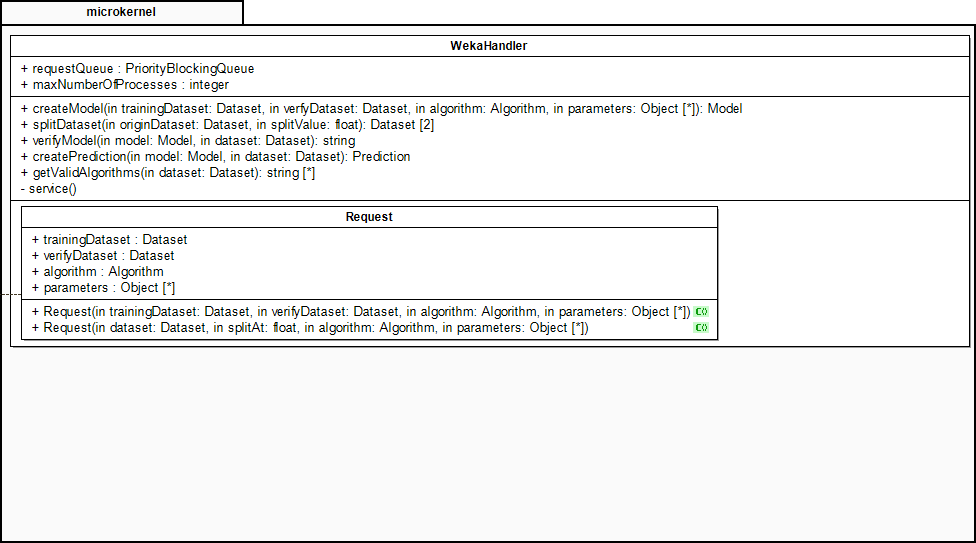
\includegraphics[width=1.0\linewidth]{Grafik/Klassendiagramme/Weka.png}
\caption{WekaHandler mit privater Request Klasse}
\end{figure}


Der WekaHandler stellt einen Wrapper um die bereits bestehende Weka-Library dar. Dieser Wrapper dient dazu, die von Weka implementierten Datenstrukturen und Methoden, zu den von uns erstellten Klassen kompatibel zu machen. Der Zugriff auf sämtliche für uns relevanten Funktionen der Library kann somit einfacher erfolgen, da ein tiefgehendes Verständnis der Selbigen nur für die Implementierung des WekaHandlers erforderlich ist, nicht aber für die Verwendung der Methoden in den restlichen Klassen.
